\documentclass[hidelinks]{thesis}

%-----------------------------------------
% Packages
%-----------------------------------------
\usepackage[a4paper,outer=0in,inner=2in,top=2in,footskip=1.2cm,textheight=25cm]{geometry}
\usepackage{graphics} % for pdf, bitmapped graphics files
\usepackage{epsfig} % for postscript graphics files
\usepackage{amsmath} % assumes amsmath package installed
\usepackage{titlesec}
\usepackage{cite}
\usepackage{color}
\usepackage{colortbl}
\usepackage{tcolorbox}
\usepackage{adjustbox}
\usepackage{multirow}
\usepackage{pgfplots}
\usepackage{csquotes}
\usepackage[linesnumbered,algoruled,boxed,lined]{algorithm2e}
\usepackage{textcomp}
\usepackage[T1]{fontenc}
\usepackage{varioref}
\usepackage{float}
\usepackage{times}
\usepackage{amssymb}
\usepackage{url}
\usepackage{textcomp}
\usepackage{sidecap}
\usepackage{verbatim} %%% for clock comments 
\usepackage{amsthm}
\usepackage{listings}
\usepackage{color} %red, green, blue, yellow, cyan, magenta, black, white
\usepackage{caption}
\usepackage{hyperref}
\usepackage[document]{ragged2e}
\usepackage{tabularx}
\usepackage[toc,page]{appendix}
\usepackage[titles]{tocloft}
\usepackage{enumitem}
%\usepackage{showframe} %show borders for debugging

\renewcommand{\cftdot}{}

\definecolor{dkgreen}{rgb}{0,0.6,0}
\definecolor{gray}{rgb}{0.5,0.5,0.5}
\definecolor{mauve}{rgb}{0.58,0,0.82}

\definecolor{lightgray}{rgb}{.9,.9,.9}
\definecolor{darkgray}{rgb}{.4,.4,.4}
\definecolor{purple}{rgb}{0.65, 0.12, 0.82}

\lstdefinelanguage{JavaScript}{
  keywords={typeof, new, true, false, catch, function, return, null, catch, switch, var, if, in, while, do, else, case, break},
  keywordstyle=\color{blue}\bfseries,
  ndkeywords={class, export, boolean, throw, implements, import, this},
  ndkeywordstyle=\color{darkgray}\bfseries,
  identifierstyle=\color{black},
  sensitive=false,
  comment=[l]{//},
  morecomment=[s]{/*}{*/},
  commentstyle=\color{purple}\ttfamily,
  stringstyle=\color{red}\ttfamily,
  morestring=[b]',
  morestring=[b]"
}

\lstset{
   language=JavaScript,
   extendedchars=true,
   basicstyle=\footnotesize\ttfamily,
   showstringspaces=false,
   showspaces=false,
     tabsize=2,
   breaklines=true,
   showtabs=false,
   captionpos=b
}


%-----------------------------------------
% From  https://tex.stackexchange.com/a/310214
%-----------------------------------------


%eformat{\chapter}[display]{\bfseries\centering}{\huge \thechapter}{1em}{\Huge #1}
%-----------------------------------------
% Start of the document
%-----------------------------------------

\titleformat{\chapter}{\centering\normalfont\huge\bfseries}{\thechapter.}{5pt}{\huge}
\titlespacing*{name=\chapter}{0pt}{-40pt}{5pt}

\begin{document}
%-----------------------------------------
% Title page
%-----------------------------------------

\begin{titlepage}
    \begin{center}
	    An Industrial Oriented Mini Project (CS70PC) Report\\
	    on\\
        {\Large  \bfseries BULK EMAIL MANAGEMENT USING SERVERLESS ARCHITECTURE}\\

	\vspace{0.2cm}
	\emph{ submitted }\\
        \emph{ in partial fulfillment of the requirements for the award of the degree of }\\
        
        \textbf{Bachelor of Technology}\\
        in\\
        \textbf{Computer Science and Engineering}\\
        by\\
        \textbf{Mr. BAZARU PRIYATHAM SAI CHAND }\\
        \textbf{(18261A0508)}\\
       \vfill 
	Under the Guidance of\\
        \textbf{Dr. A. Nagesh}\\
        \textbf{(Professor)}\\

        \vfill
	\vspace{0.4cm}
        \begin{figure}[h]
            \centering
            
\includegraphics[width=39mm]{figures/mgit_logo_1.png}
        \end{figure}

        \vfill
        Department of Computer Science and Engineering\\
        \textbf{MAHATMA GANDHI INSTITUTE OF TECHNOLOGY}\\
    \small \text{(Affiliated to Jawaharlal Nehru Technological University, Hyderabad)}\\
        Hyderabad 500075, Telangana (India).\\
        \small \text{2021-2022}\\
    \end{center}
\end{titlepage}



%-----------------------------------------
% Declaration, Acknowledgement
%-----------------------------------------
\pagenumbering{roman}
\addcontentsline{toc}{chapter}{CERTIFICATE}
\justifying
\begin{center}
    \Large\textbf{ MAHATMA GANDHI INSTITUTE OF TECHNOLOGY}\\    
    \small \text{(Affiliated to Jawaharlal Nehru Technological University, Hyderabad)}\\
    \text{GANDIPET, HYDERABAD - 500 075. Telangana} \\

    \vspace{0.5cm}
    \Large \textbf{CERTIFICATE}
    \begin{figure}[h]
        \centering
        
\includegraphics[width=40mm]{figures/mgit_logo_1.png}
    \end{figure}
\end{center}
    \small
    This is to certify that the thesis entitled \textbf{Bulk Email Management Using Serverless Architecture} is being submitted by \textbf{Bazaru Priyatham Sai Chand} bearing \textbf{ Roll no. 18261A0508 } in partial fulfillment for the award of \textbf{B.Tech} in \textbf{Computer Science and Engineering} to \textbf{Jawaharlal Nehru Technological University, Hyderabad} is a record of bonafide work carried out by him under my guidance and supervision.
    
    \par
    \noindent
The results embodied in this project have not been submitted to any other University or Institute for the award of any degree or diploma. 
    
    \vspace{2cm}


    \noindent
	    \begin{minipage}[t]{0.2\textwidth}
			    \text{Project Guide}\\
			    \textbf{Dr. A. Nagesh}\\
		    \text{Professor}\\
	    \end{minipage}
	    \hfill
	    \begin{minipage}[t]{0.2\textwidth}
			    \text{Head of Department}\\
			    \textbf{Dr. C.R.K Reddy}\\
			    \text{Professor}
	    \end{minipage}


    \vspace{3cm}
\begin{center}
    \textbf{External Examiner}
\end{center}
 
\chapter*{DECLARATION}
\addcontentsline{toc}{chapter}{DECLARATION}

\doublespace
\doublespace

\qquad 

\vspace{2cm}
\justifying

\noindent
This is to certify that the work reported in this project titled \textbf{"Bulk Email Management using Serverless Architecture"} is a record of work done by me in the \textbf{Department of Computer Science and Engineering, Mahatma Gandhi Institute of Technology, Hyderabad.} \par

\noindent
No part of the work is copied from books/journals/internet and wherever the portion is taken, the same has been duly referred in the text. The report is based on the work done entirely by me and not copied from any other source.



\vskip 2cm
\noindent{
   \hfill 
    \large \textbf{B. PRIYATHAM SAI CHAND}\\

}

\vskip -1cm
\noindent{
   \hfill 
    \large \textbf{(18261A0508)}\\

}
\par

\chapter*{ACKNOWLEDGEMENT}
\addcontentsline{toc}{chapter}{ACKNOWLEDGEMENT}

\doublespace

\noindent
I would like to express my sincere thanks to \textbf{Dr.K.Jaya Shankar, Principal,MGIT}, for providing the working facilities in college.\\

\noindent
I wish to express my sincere thanks and gratitude to \textbf{Dr.C.R.K Reddy, Professor and HOD,} Department of CSE, MGIT for all the timely support and valuable suggestions during the period of project. \\

\noindent
I am extremely thankful to \textbf{Dr.B.Prasanthi, Sr Assistant Professor and Ms.D.Deepika, Assistant Professor,} Department of CSE, MGIT, mini project coordinators for their encouragement and support throughout the project. \\

\noindent
I am extremely thankful and indebted to my internal guide \textbf{Dr. A. Nagesh, Professor}, Department of CSE, for his constant guidance, encouragement and moral support throughout the project. \\

\noindent
Finally, I would also like to thank all the faculty and staff of CSE Department who helped me directly or indirectly, for completing this project.
\vskip 2cm
\noindent{
   \hfill 
    \large \textbf{B. PRIYATHAM SAI CHAND}\\ \rule{1cm}{0pt}
}
\vskip -1cm
\noindent{
   \hfill 
    \large \textbf{(18261A0508)}\\

}

\par\newpage

%----------------------------------------------
% Table of contents, list of figures and tables
%----------------------------------------------

%- capitalizing contents 
\let\mtcontentsname\contentsname
\renewcommand\contentsname{TABLE OF CONTENTS}
\renewcommand*\listfigurename{LIST OF FIGURES}  %- capitalize list of figures
\renewcommand*\listfigurename{LIST OF FIGURES}  %- capitalize list of figures
\renewcommand*\listtablename{LIST OF TABLES} 

\tableofcontents
\newpage
\listoffigures
\listoftables

%-----------------------------------------
% Abstract
%-----------------------------------------
%\titleformat{\chapter}[display]
%{\centering\normalfont\huge\bfseries}{\chaptertitlename~\thechapter}{15pt}{\huge}
%\titlespacing*{\chapter}{0pt}{0pt}{10pt}
%\titlespacing*{name=\chapter,numberless}{0pt}{-40pt}{10pt}
%\renewcommand{\@makeschapterhead}[1]{%
%%  \vspace*{50\p@}%
%  \vspace*{20\p@}%
%  {\parindent \z@ \raggedright
%    \normalfont
%    \interlinepenalty\@M
%    \Huge \bfseries  #1\par\nobreak
%%    \vskip 40\p@
%    \vskip 20\p@
%  }}
\chapter*{ABSTRACT}
\addcontentsline{toc}{chapter}{ABSTRACT}
\thispagestyle{empty}
\justifying

Email has become one of the most important means of communications.Sending emails through conventional software like Gmail is limited to a mere thousands which is not sufficient to fit into the business needs and managing the insights of sent emails is crucial to companies to further enhance their approach. Serverless computing is any computing platform that hides server usage from developers and runs code on-demand automatically scaled and billed only for the time the code is running \cite{castro2019rise}.This reduces the time and knowledge required to deploy pieces of software while offering significant reduction in pricing compared to hosting the software on dedicated hardware.\par

\vspace{0.2cm}
\noindent
Various cloud platforms such as Amazon Web Services (AWS), Microsoft Azure and Google Cloud Platform have adapted to this way of thinking making it easily accessible.A robust serverless architecture for sending bulk emails of the magnitude of thousands to millions using scalable model which is implemented using AWS lambda\cite{awslambda} and Simple Email Service(SES) for the SMTP protocol.\par 

\vspace{0.2cm}
\noindent
Challenges such as able to trace the bounce emails as well as the statistics for the emails sent. The prototype is built using the ReactJS framework along with underlying services from AWS. These tightly integrated services offer the best way to simulate the architecture and help in sending customized for every recipient based on email templates along with storing bounce emails. The effectiveness of the scalability offered by the architecture is analyzed using X-ray traces to simulate and test the bottlenecks and how to overcome them is discussed. With serverless technology, the cloud provider abstracts away the server management, provisioning servers with fine granularity, on demand, and with a pay-per-use model\cite{eismann2020serverless}. \par


\vspace{0.2cm}
\noindent
This project proposes an architecture for sending and management of the emails through serverless application using the AWS services and its implementation using a javascript based frontend application.

\par
\vspace{0.1cm}
\noindent
\textbf{Keywords :} Serverless,bounce emails,scalability.


%-----------------------------------------
% Chapters
%-----------------------------------------

\pagenumbering{arabic}
\chapter{INTRODUCTION}
\label{intro}

\justifying

\section{Overview}
The bulk email management system is used to send emails of magnitude in thousands and more and broadcast the message to multiple email addresses with a single operation. All the required fields such as the senders’ email addresses, subject, the html body and to addresses are selected and the sending is initiated with a button. Upon successful sending to the API endpoint the emails are processed and send through the AWS simple email services to all the users and the emails that were bounced are returned after the sending operation.It makes use of a Javascript based framework called ReactJS to input the fields and send it to the API hosted on the AWS service where an array of services are used to scale and perform the sending and retrieving of bounces.\par
\noindent
In this project, the functions to send and manage emails using serverless functions is implemented and an application is created for usability. \section{Different Kinds of Services}

The serverless functionalities utilized in this project are:

\subsection{Lambda Function}
AWS Lambda is a serverless, event-driven compute service that lets you run code for virtually any type of application or backend service without provisioning or managing servers. You can trigger Lambda from over 200 AWS services and software as a service (SaaS) applications, and only pay for what you use.\cite{awslambda}

\subsection{Simple Email Service
}

Amazon Simple Email Service (SES) is a cost-effective, flexible, and scalable email service that enables developers to send mail from within any application. You can configure Amazon SES quickly to support several email use cases, including transactional, marketing, or mass email communications. Amazon SES's flexible IP deployment and email authentication options help drive higher deliverability and protect sender reputation, while sending analytics measure the impact of each email. With Amazon SES, you can send email securely, globally, and at scale.\cite{awsses}

\subsection{Simple Notification Service}
%\begin{figure}[h]
%            \centering
%            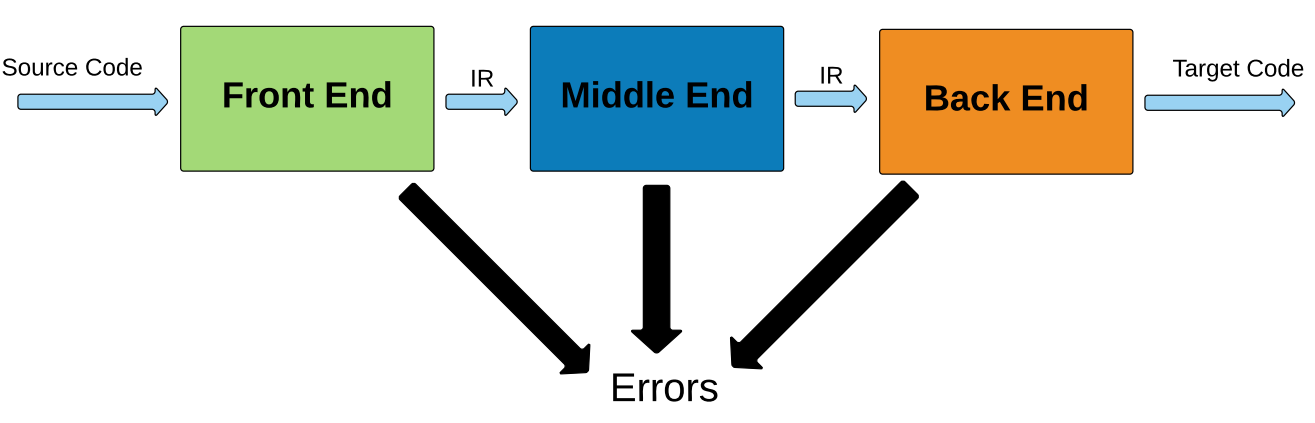
\includegraphics[width=150mm]{figures/multi_pass_compile.png}
%            \caption{Multi Pass Compiler}
%            \label{fig:multi-pass-compiler}
%\end{figure}
%
%Figure \ref{fig:multi-pass-compiler} shows a multi pass compiler which processes the source code or syntax tree of a program several times. It divides a large program into multiple small programs and processes them. It develops multiple intermediate codes. Each of the multi pass takes output of the previous pass as an input. So it requires less memory. It is also known as \textbf{Wide Compiler}. 

Amazon Simple Notification Service (Amazon SNS) is a fully managed messaging service for both application-to-application (A2A) and application-to-person (A2P) communication. The A2A pub/sub functionality provides topics for high-throughput, push-based, many-to-many messaging between distributed systems, microservices, and event-driven serverless applications. Using Amazon SNS topics, your publisher systems can fanout messages to a large number of subscriber systems, including Amazon SQS queues, AWS Lambda functions, HTTPS endpoints, and Amazon Kinesis Data Firehose, for parallel processing. The A2P functionality enables you to send messages to users at scale via SMS, mobile push, and email.\cite{awssns}
\subsection{Simple Queue Service}
Amazon Simple Queue Service (SQS) is a fully managed message queuing service that enables you to decouple and scale microservices, distributed systems, and serverless applications. SQS eliminates the complexity and overhead associated with managing and operating message-oriented middleware, and empowers developers to focus on differentiating work. Using SQS, you can send, store, and receive messages between software components at any volume, without losing messages or requiring other services to be available. 

SQS offers two types of message queues. Standard queues offer maximum throughput, best-effort ordering, and at-least-once delivery. SQS FIFO queues are designed to guarantee that messages are processed exactly once, in the exact order that they are sent. We use the FIFO queue to process the emails to be sent exactly once and make sure duplication does not occur within the list of emails.\cite{awssqs}

\subsection{API Gateway
}Amazon Application Program Interface (API) Gateway is a fully managed service that makes it easy for developers to create, publish, maintain, monitor, and secure APIs at any scale. APIs act as the "front door" for applications to access data, business logic, or functionality from your backend services. Using API Gateway, you can create Representational State Transfer (REST)ful APIs and WebSocket APIs that enable real-time two-way communication applications. API Gateway supports containerized and serverless workloads, as well as web applications.\cite{awsapi}
\subsection{CloudWatch
}Amazon CloudWatch is a monitoring and observability service built for DevOps engineers, developers, site reliability engineers (SREs), IT managers, and product owners. CloudWatch provides you with data and actionable insights to monitor your applications, respond to system-wide performance changes, and optimize resource utilization. CloudWatch collects monitoring and operational data in the form of logs, metrics, and events. You get a unified view of operational health and gain complete visibility of your AWS resources, applications, and services running on AWS and on-premises. You can use CloudWatch to detect anomalous behavior in your environments, set alarms, visualize logs and metrics side by side, take automated actions, troubleshoot issues, and discover insights to keep your applications running smoothly.\cite{awscloudwatch}
\subsection{X-ray}
AWS X-Ray helps developers analyze and debug production, distributed applications, such as those built using a microservices architecture. With X-Ray, you can understand how your application and its underlying services are performing to identify and troubleshoot the root cause of performance issues and errors. X-Ray provides an end-to-end view of requests as they travel through your application, and shows a map of your application’s underlying components. You can use X-Ray to analyze both applications in development and in production, from simple three-tier applications to complex microservices applications consisting of thousands of services.\cite{awsxray}

\newpage

\section{Problem Definition}

Given a set of emails in the form of comma separated values with their respective subjects and email content send the respective emails to everyone on the list without provisioning any form of server and track the information about the sent emails such as the bounced emails, delivered, opened and bounce rate of the from address using a dashboard.


\section{Proposed System}

The proposed system comprises of an AWS system that can serve as a serverless backend that is invoked using a REST API request made from a javascript based frontend made using the library of ReactJS.




\section{Requirements Specification}
\subsection{Software Requirements}
\begin{enumerate}
    \item Software : Any javascript enabled internet browser,Node.js 14.x .
    \item Languages : Javascript
\end{enumerate}


\subsection{Hardware Requirements}
\begin{enumerate}
    \item Random Access Memory: 2 GB.
    \item Storage: 500MB for internet browser.
\end{enumerate}

%\newgeometry{a4paper,outer=0in,inner=2in,top=1in,footskip=2in}
%\titleformat{\chapter}
%{\centering\normalfont\huge\bfseries}{\thechapter.}{15pt}{\huge}
%\titlespacing*{name=\chapter}{0pt}{-40pt}{10pt}
\chapter{LITERATURE SURVEY}
%\titleformat{\chapter}[display]{\normalfont\huge\bfseries}{\thechapter.\chaptername}{20pt}{\Huge}
%\titlespacing*{name=\chapter}{0pt}{-50pt}{10pt}
\label{ch:literature_survey}

In literature survey I have investigated various researches on this particular domain and some of them are as follows :-

\begin{enumerate}[wide, labelwidth=!, labelindent=0pt]
    \item \textbf{Serverless Applications: Why, When, and How?} \cite{eismann2020serverless}

  Serverless computing shows good promise for efficiency and ease-of-use. Yet, there are only a few, scattered and sometimes conflicting reports on questions such as Why do so many companies adopt serverless?, When are serverless applications well suited?, and How are serverless applications currently implemented? To address these questions, we analyze 89 serverless applications from open-source projects, industrial sources, academic literature, and scientific computing—the most extensive study to date.     
    \item \textbf{Serverless Electronic Mail } \cite{goodell2020serverless}


  We describe a simple approach to peer-to-peer electronic mail that would allow users of ordinary workstations and mobile devices to exchange messages without relying upon third-party mail server operators. Crucially, the system allows participants to establish and use multiple unlinked identities for communication with each other. The architecture leverages ordinary SMTP \cite{rfc5322} for message delivery and Tor \cite{dingledine2004tor} for peer-to-peer communication. The design offers a robust, unintrusive method to use self-certifying Tor onion service names to bootstrap a web of trust based on public keys for end-to-end authentication and encryption, which in turn can be used to facilitate message delivery when the sender and recipient are not online simultaneously. We show how the system can interoperate with existing email systems and paradigms, allowing users to hold messages that others can retrieve via IMAP \cite{rfc3501}  or to operate as a relay between system participants and external email users. Finally, we show how it is possible to use a gossip protocol to implement mailing lists and how distributed ledger technology might be used to bootstrap consensus about shared knowledge among list members.
    \item \textbf{Tracking Causal Order in AWS Lambda Applications} \cite{lin2018tracking}
    
   Serverless computing is a new cloud programming and deployment paradigm that is receiving wide-spread uptake. Serverless offerings such as Amazon Web Services (AWS) Lambda, Google Functions, and Azure Functions automatically execute simple functions uploaded by developers, in response to cloud-based event triggers. The serverless abstraction greatly simplifies integration of concurrency and parallelism into cloud applications, and enables deployment of scalable distributed systems and services at very low cost. Although a significant first step, the serverless abstraction requires tools that software engineers can use to reason about, debug, and optimize their increasingly complex, asynchronous applications. Toward this end, we investigate the design and implementation of GammaRay, a cloud service that extracts causal dependencies across functions and through cloud services, without programmer intervention. We implement GammaRay for AWS Lambda and evaluate the overheads that it introduces for serverless micro-benchmarks and applications written in Python.     
    \item \textbf{Serverless Computing: Design, Implementation, and Performance} \cite{mcgrath2017serverless}
    
  We present the design of a novel performance- oriented serverless computing platform implemented in .NET, deployed in Microsoft Azure, and utilizing Windows containers as function execution environments. Implementation challenges such as function scaling and container discovery, lifecycle, and reuse are discussed in detail. We propose metrics to evaluate the execution performance of serverless platforms and conduct tests on our prototype as well as AWS Lambda, Azure Functions, Google Cloud Functions, and IBM’s deployment of Apache OpenWhisk. Our measurements show the prototype achieving greater throughput than other platforms at most concurrency levels, and we examine the scaling and instance expiration trends in the implementations. Additionally, we discuss the gaps and limitations in our current design, propose possible solutions, and highlight future research.     
    \item \textbf{Be wary of the economics of "Serverless" Cloud Computing} \cite{eivy2017wary}
    
   In standard cloud computing, dedicated hard- ware is replaced by dynamically allocated, pay-per- use resources, such as virtual servers. Although called “pay-per-use,” these resources are typically billed based on allocation, not on actual use, potentially leading to a customer paying more than necessary. In “serverless,” no resources are typically allocated or chargeable until a function is called. It’s like the difference between a rental car and a taxi: you will be charged for the rental car even if you park it for a week, unlike a taxi. Moreover, some cloud providers are offering seemingly massive amounts of serverless computing at no charge. This holds the promise of the most efficient processing possible—for free or at least what seem to be attractive prices. Moreover, serverless fits with the modern approach to application construction—composing microservices rather than building hard-to-manage and scale monolithic applications. However, as with many things, the devil is in the details and the economic benefits of serverless computing heavily depend on the execution behavior and volumes of the application workloads. In the same way that pennies per day can add up to thousands of dollars eventually, low “per hit” prices can not only add up as transaction volumes increase, but can make serverless economics unattractive relative to what have now become more traditional approaches,such as virtual machines or even dedicated hardware. 


\item \textbf{Honorable Mention: Serverless architecture-a revolution in cloud computing} \cite{rajan2018serverless}

\noindent
Emergence of cloud computing as the inevitable IT computing paradigm, the perception of the compute reference model and building of services has evolved into new dimensions. Serverless computing is an execution model in which the cloud service provider dynamically manages the allocation of compute resources of the server. The consumer is billed for the actual volume of resources consumed by them, instead paying for the pre-purchased units of compute capacity. This model evolved as a way to achieve optimum cost, minimum configuration overheads, and increases the application's ability to scale in the cloud. The prospective of te serverless compute model is well conceived by the major cloud service providers and reflected in the adoption of serverless computing paradigm. This review paper presents a comprehensive study on serverless computing architecture and also extends an experimentation of the working principle of serverless computing reference model adapted by AWS Lambda. The various research avenues in serverless computing are identified and presented.
\end{enumerate}

\begin{table}[H]
	%\rowcolors{1,3,6}{mygreen!20}{white}

\begin{tabular}{|p{1.2em}|p{2.6em}|p{3.0em}|p{7.5em}|p{6em}|p{4.5em}|p{5.5em}|} 
\hline
S.no & Publish Year & Author & Title & Application & Advantage & Disadvantages \\
\hline
1. & 2020 &Simon Eismann et al.&\textbf{Serverless Applications:
Why, When, and How? } & computing is isolated till it's completion &Describes case study for serverless backend& Only covers studies on adaption rather than success rate\\ 
\hline
2. & 2020 &Geoffrey Goodell&\textbf{Serverless Electronic Mail } & P2P network for email management & Gives better idea of SMTP in serverless networks &Considers a decentralized network based on Tor.\\ 
\hline
3. & 2018& Wei-Tsung Lin et al.&\textbf{Tracking Causal Order in AWS Lambda Applications}&  performance benchmarks for using lambda with various other services.& Detailed analysis on compatibility and what to expect upon combining.& Uses a niche tool called Gammaray which is superseded by X-ray traces.\\ 
\hline

4. & 2017& McGrath et al.  & \textbf{Serverless Computing: Design, Implementation, and Performance} &  Compare and contrast various providers and approach needed & gives model architectures and design stragies  & Provides solutions based on containers.\\ 
\hline
5. & 2017 & Adam Eivy & \textbf{Be wary of the economics of "Serverless" Cloud Computing} & Explains the cost attributed with this technology & In detail about Scalability vs Economics & Doesn't cover larger payload scenarios\\ 
\hline
\end{tabular}
\caption{Summary of literature survey}
\end{table}


\chapter{DESIGN METHODOLOGY OF BULK EMAIL MANAGEMENT SYSTEM}
\label{design_meth}

\section{UML Diagrams}
The Unified Modelling Language (UML) is a standard language for writing software blueprints. UML can be used for:

\begin{itemize}
  \item \textbf{Specifying}: It is a blueprint created by an architect prior to the construction.
  \item \textbf{Visualizing} : Visualizing is concerned with deep analysis of system to be constructed.
  \item \textbf{Constructing} : Modelling also provide us mechanism which are essential while
constructing a system.
 \item \textbf{Documenting} : Finally, modelling justifies its importance by applying all its credentials
to be bounded in a piece of paper referred as document. 

\end{itemize}

The UML is a language which provides vocabulary and the rules for combining words in that vocabulary for the purpose of communication. A modelling language is a language whose
vocabulary and the rules focus on the conceptual and physical representation of a system. Modelling yields an understanding of a system.

Three types of diagrams are shown to propose the design and depict the methodology that is implemented by using the appropriate tools.

\subsection{Use Case Diagram}

\begin{figure}[H]
            \centering
            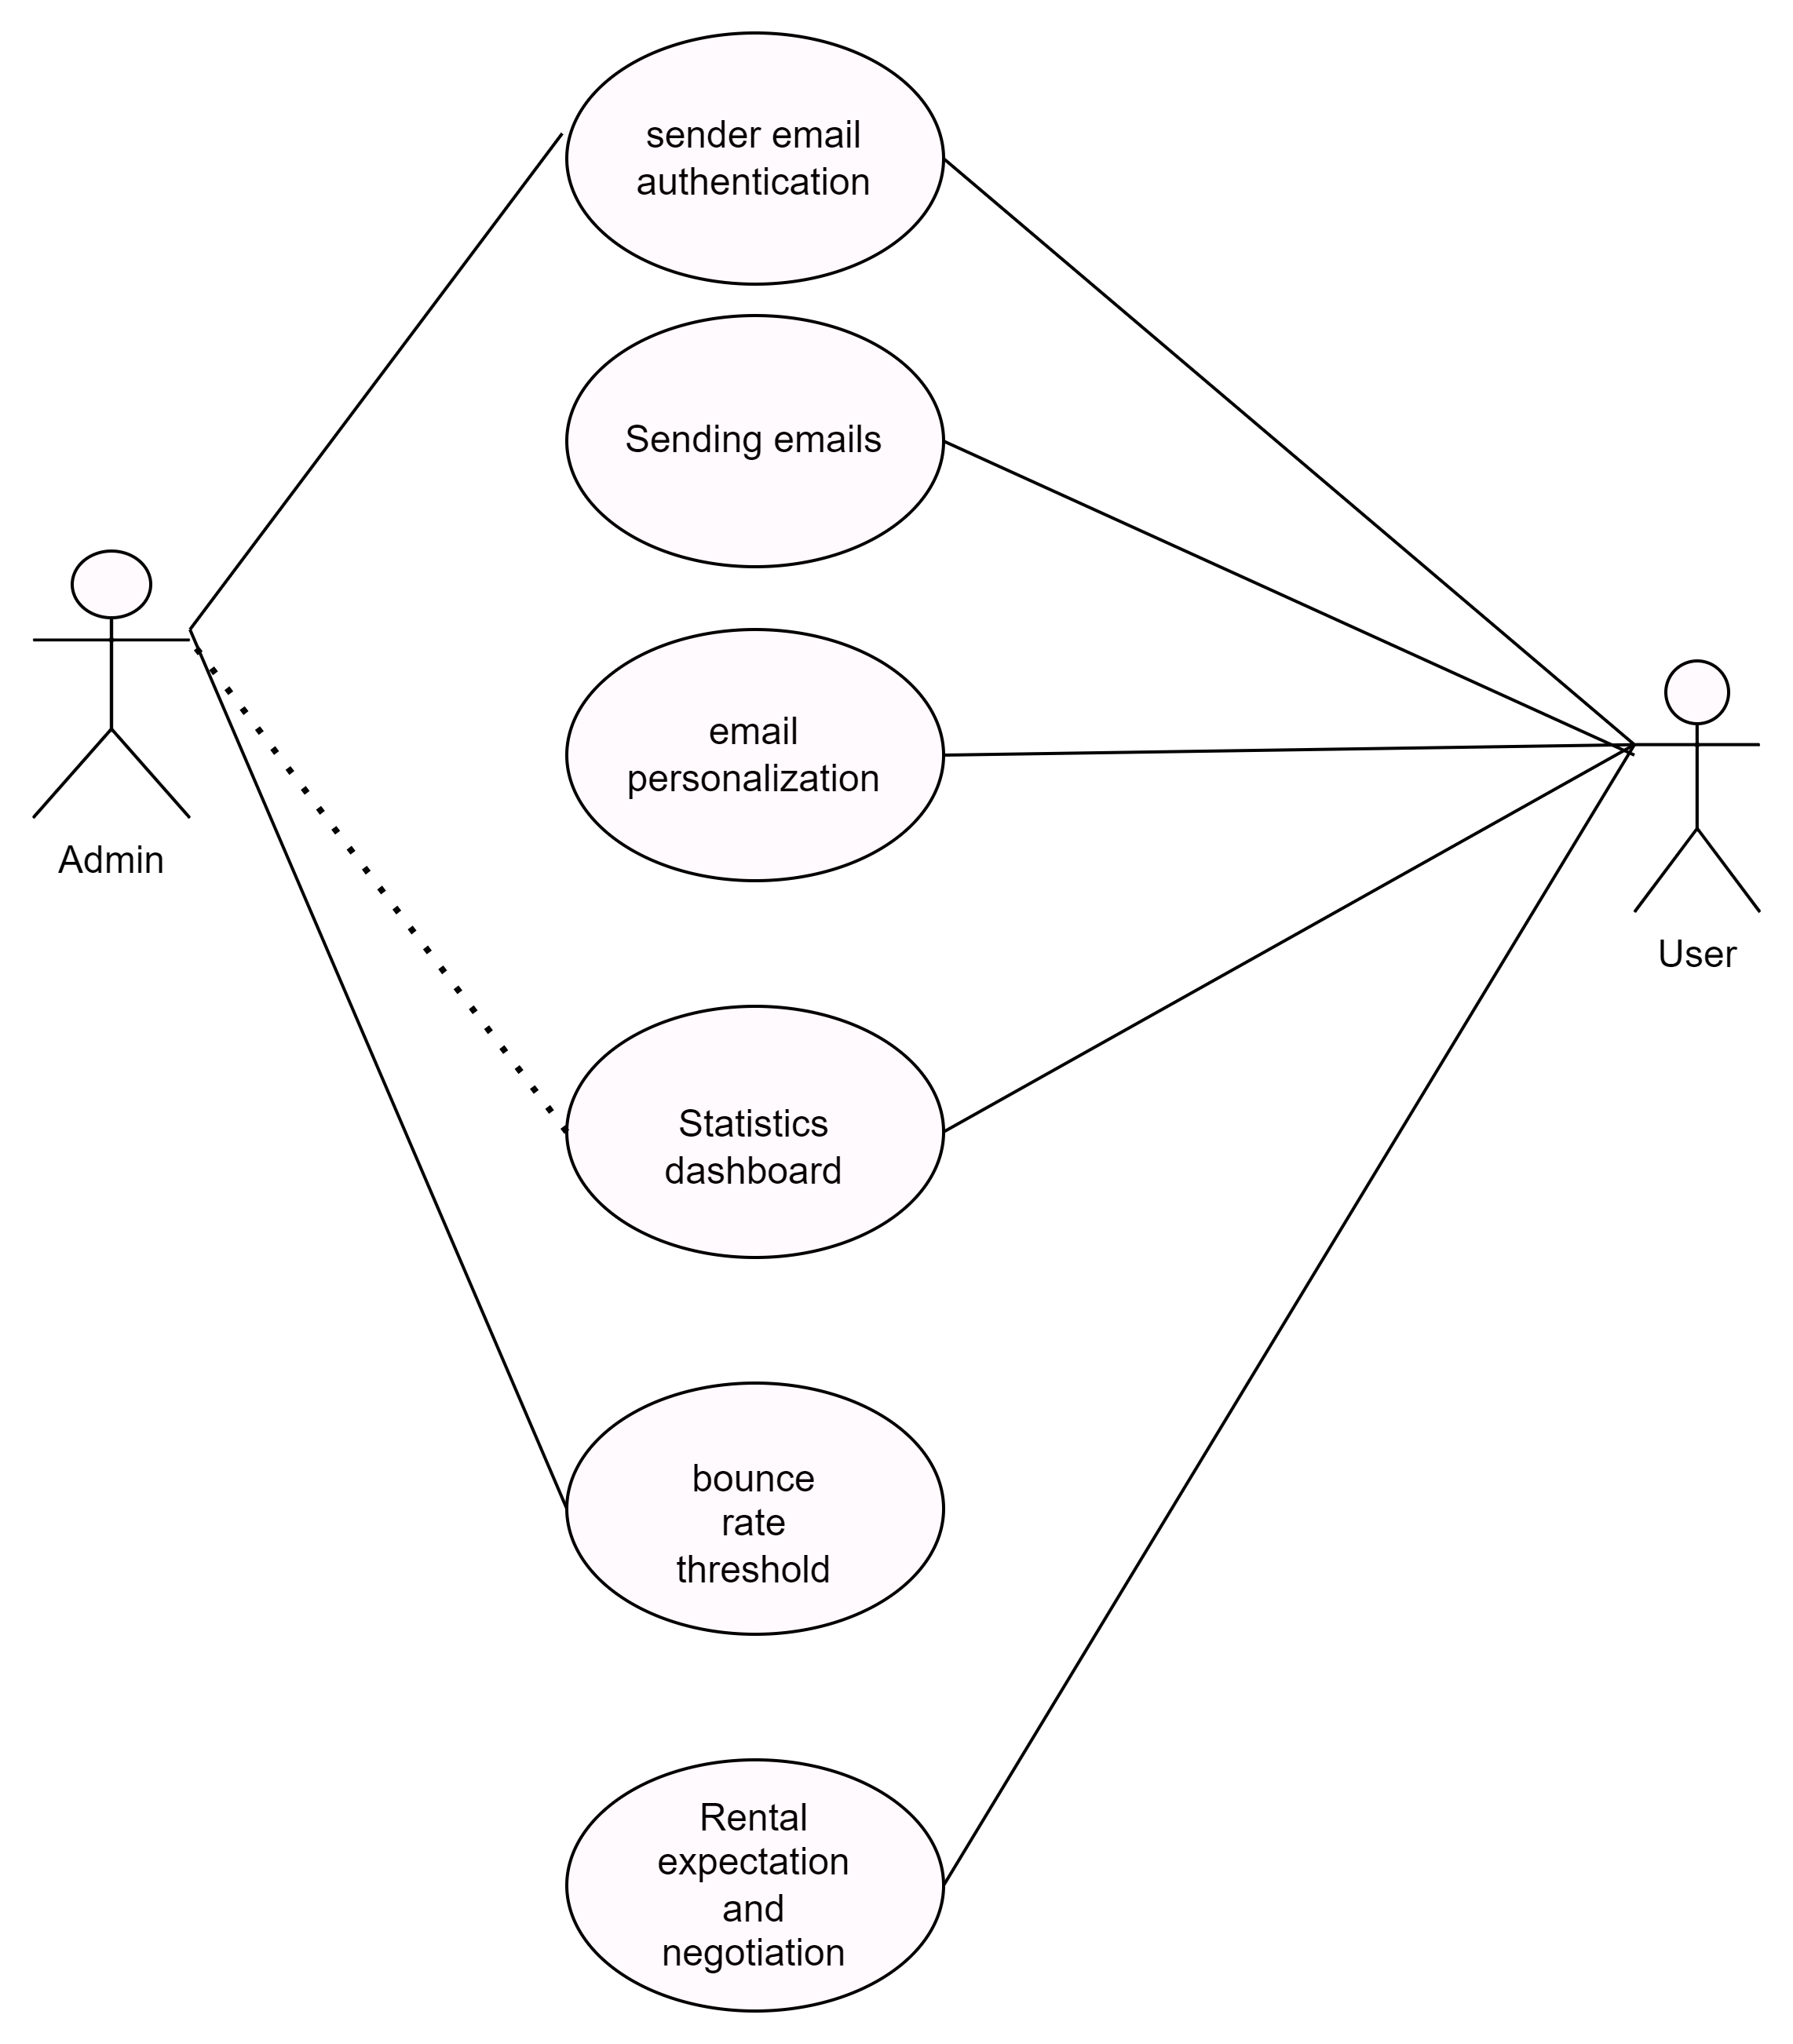
\includegraphics[width=160mm, height=100mm]{figures/use_case.png}
            \caption{Use case Diagram}
            \label{fig:use-case-diagram}
\end{figure}

Use case diagrams are used to gather the requirements of a system including internal and external influences. These requirements are mostly design requirements. So, when a system
is analyzed together its functionalities use cases are prepared and actors are identified. 

In Figure \ref{fig:use-case-diagram}, the user gives in Input Program to the compiler and is able to view the outcomes of Syntax, Lexical analysis phases of the compilation process (compilation errors if any in the source code).

 

\section{Data Flow Diagram}

A data-flow diagram is a way of representing a flow of data through a process or a system (usually an information system). The DFD also provides information about the outputs and inputs of each entity and the process itself. A data-flow diagram has no control flow, there are no decision rules and no loops. Specific operations based on the data can be represented by
a flowchart. 

For each data flow, at least one of the endpoints (source and / or destination) must exist in a process. The refined representation of a process can be done in another data-flow diagram, which subdivides this process into sub-processes.



\begin{figure}[H]
            \centering
            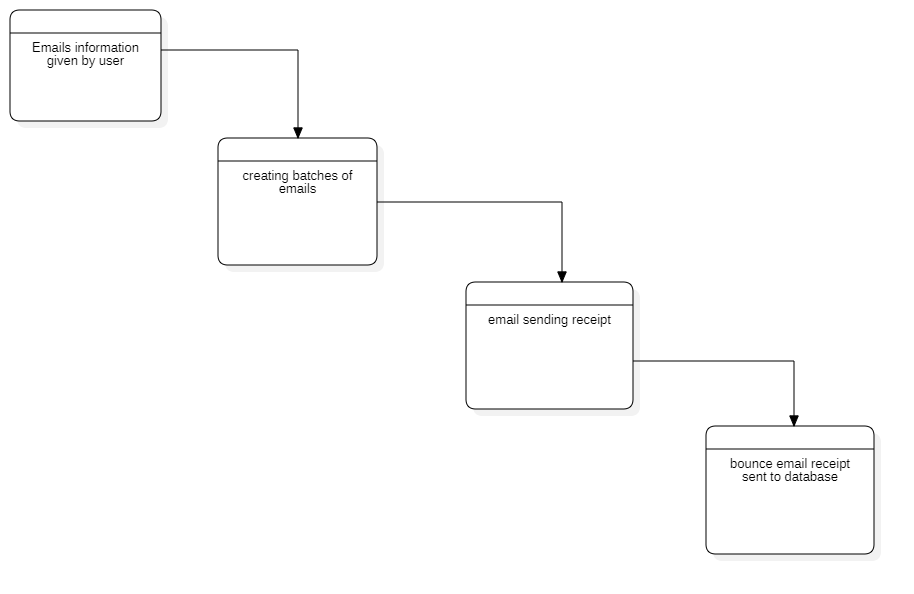
\includegraphics[width=160mm]{figures/data_flow_diagram.png}
            \caption{Data Flow Diagram of bulk email management system}
	    \label{fig:data-flow-diagram}
\end{figure}


The data flow diagram displayed in Figure \ref{fig:data-flow-diagram} shows how the data that is entered by the user is processed till the sending of emails and further finding the bounce emails data and how they are stored finally in a database.

\section{Architecture diagram}

Architecture diagram shows how various components that exists in a network work together and are integrated with other services. User interaction to output the various methods and services used and their correlation is depicted in this diagram.

The components used can be instances of a component and the sequence in which they need to be connected to successfully achieve the desired output is shown here.

\begin{figure}[H]
            \centering
            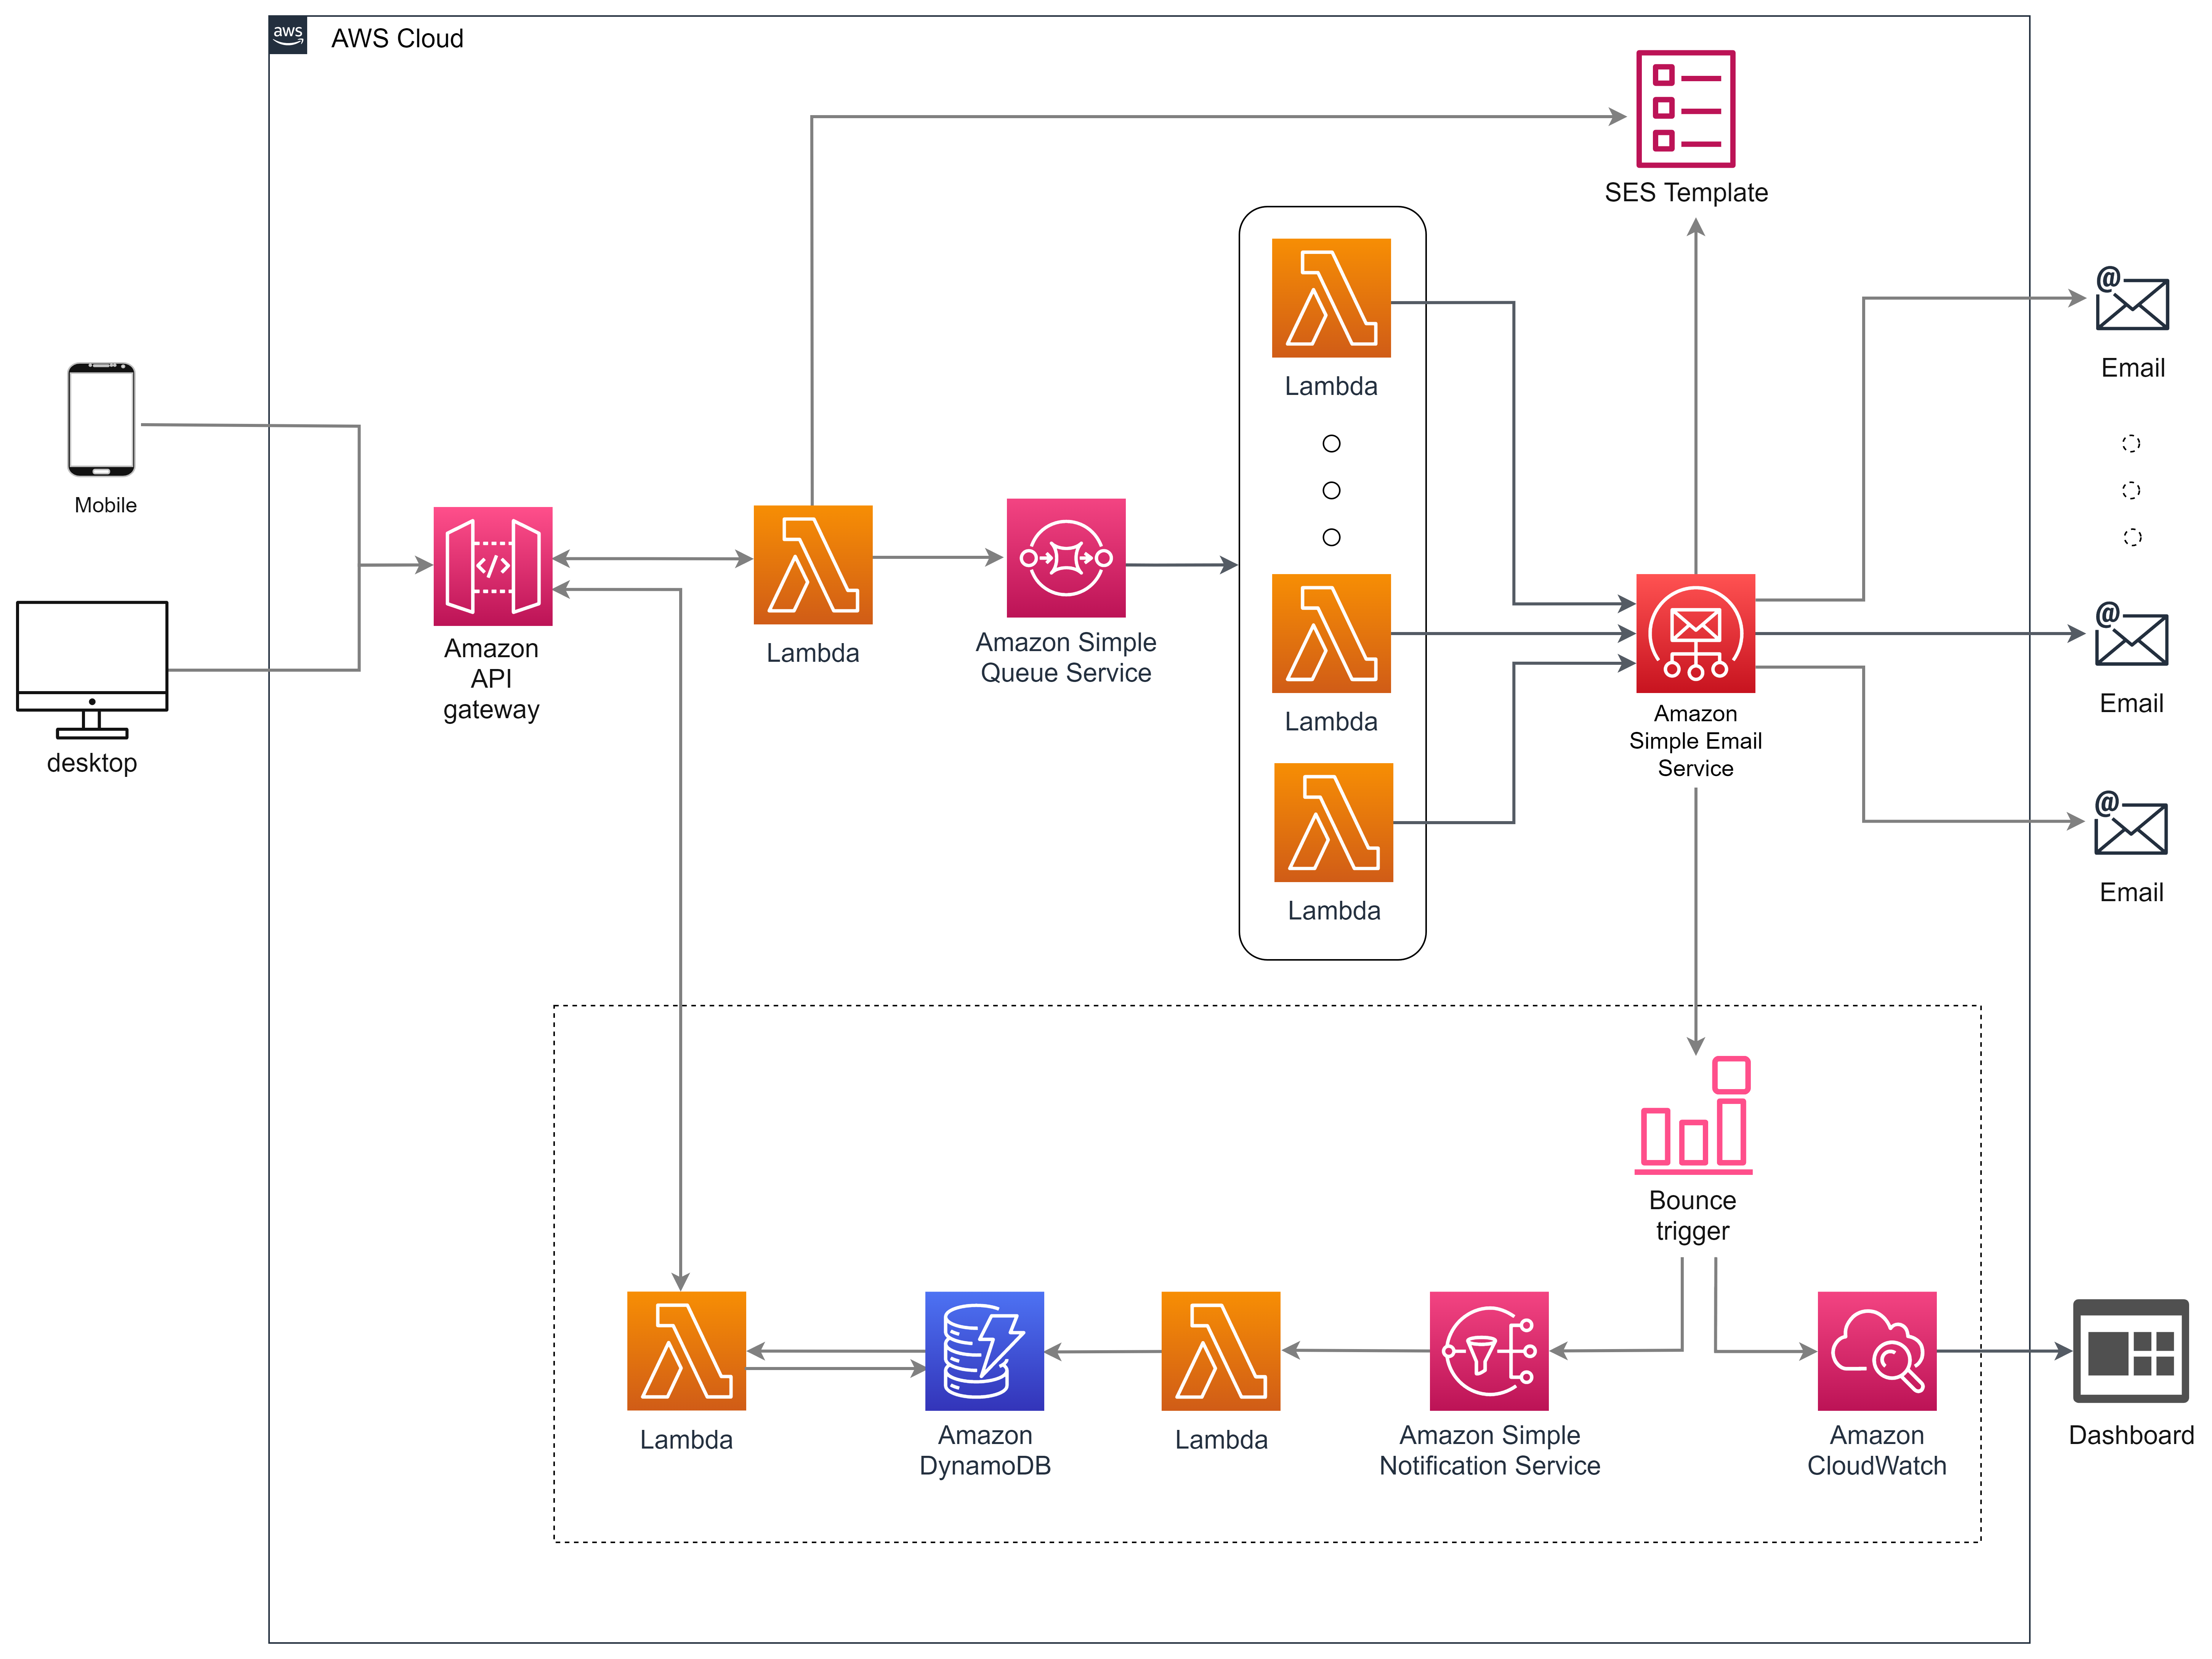
\includegraphics[width=160mm]{figures/architect.png}
            \caption{AWS architecture of bulk email management system}
	    \label{fig:architect}
\end{figure}


The data flow diagram displayed in Figure \ref{fig:architect} shows how the data that is entered by the user is processed till the sending of emails and further finding the bounce emails data and how they are stored finally in a database.

The architecture is based a few constraints from the SES service and other bottlenecks that affect the sending of emails. The SES through which the emails are initially sent through sandbox to test and later needs to be upgraded by the AWS authority to permit the user to request increase in the number of emails to be sent. For the purpose of this architecture 50,000 emails have been requested which was granted by the authority.
\begin{itemize}
	\item 14 emails/second
	\item 50,000 emails per day
	\item request data 5kb
\end{itemize}


\chapter{IMPLEMENTATION}
\label{ch:lex_yacc}


The architecture demonstrated in the Fig 1 with the main functionalities include sending the emails and tracking the bounces. Initially, all the data sent to the lambda using the API gateway which handles the request and response for the whole operation. Upon reaching the lambda, JavaScript Object Notation (JSON) objects from the string parameters preprocessed, the html part of the email along with the subject made into SES templates accessed by other lambdas and the emails batched no more than 50 emails per batch and placed in a Simple queue Service[5] queue. The ordering of the messages is important hence, we use a First In First Out queue, which triggers another lambda that sends emails to all the 50 recipients using a templated email function by accessing the template that we created earlier. We set a flag to mark the end of the batches deleting the template by the end of the execution.


\section{Frontend}

The web application is used to fill and send the emails to all the users at the same time. The application is built using ReactJS library and bootstrap library to style the web page. A basic layand intuitive layout is given considering the web application is mostly used as internal software within an organization or various organizations as a service. 
The fields that need to be filled are

\begin{enumerate}
	\item \textbf{Emails} - Comma seperated values of the emails with spaces and that follows the standard email format.  
	\item \textbf{Names} - Comma separated values of the names corresponding to the emails above it is not a required field. The names will be made into empty strings in the preprocessing.
	\item \textbf{Subject} - String value giving the subject. It is a mandatory field.
	\item \textbf{html} - The email body that is sent to the users. It is interpreted as html code when sent to the lambda function.
	\item \textbf{Sender's email} - The senders email needs to be verified by OTP with AWS console before sending the emails. After an email is verified it is added into the dropdown by the admin. Any one of the verified emails can be used.
\end{enumerate}


\begin{figure}[H]
            \centering
            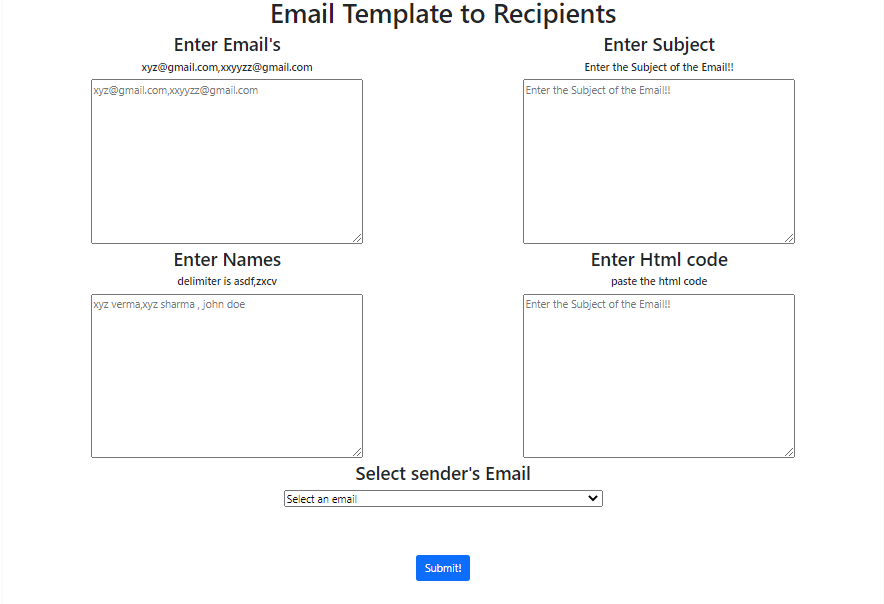
\includegraphics[width=150mm,height=90mm]{figures/frontend_1.png}
            \caption{Frontend Web Application}
            \label{fig:frontend-web}
\end{figure}

In Figure \ref{fig:frontend-web} The web application made using the styling packages is shown. All the respective fields that were mentioned before can be filled out by the user and click on submit to initialize the preprocessing and sending of data to the serverless functions.


\begin{figure}[H]
            \centering
            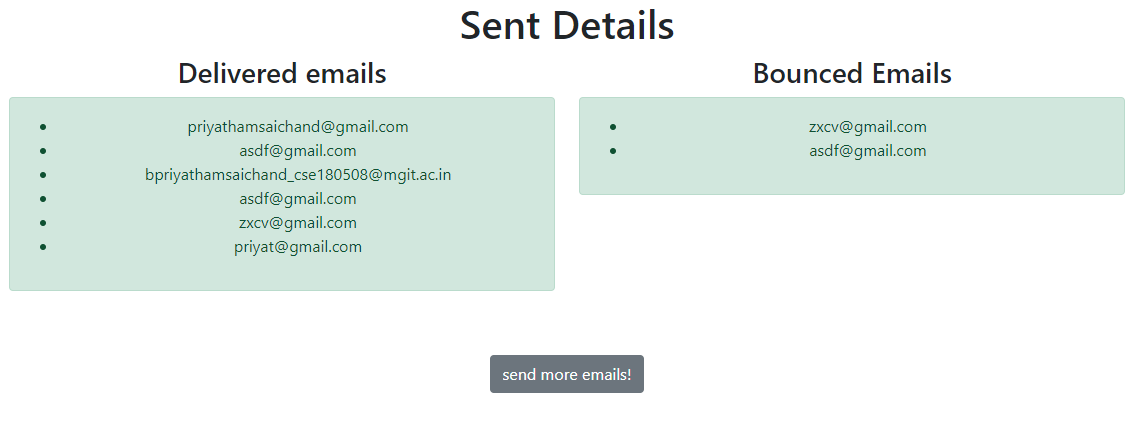
\includegraphics[width=130mm,height=90mm]{figures/result_1.png}
            \caption{Output webpage}
            \label{fig:frontend-output}
\end{figure}


In Figure \ref{fig:frontend-output} The output webpage that is returned after the emails are sent is shown.  

\section{Serverless Functions}
To implement the business logic that is present in the backend. Four lambda functions where created to be used to send and manage the bounces that are generated. Their functionalities are described as follows.

\subsection{email\_batcher}

The purpose of this function is to receive the POST request payload with all the required information such as emails, names, sender's email and subject. It creates the email template with the HTML and sender's email. As per the constraints mentioned in design and methodology, upto 50 emails are batched into a single JSON object and sent into the FIFO queue. All the preprocessing of the string data to json objects is done in this function and is the first function executed with every API call. This lambda function is invoked as a trigger with API gateway used to handle the API endpoints of the application. 


\subsection{sqs\_mailer}

This function is used to send the emails obtained from the FIFO queue. It uses the template that was created by email\_batcher and uses the SES service to send the emails to 50 email addresses along with their names using the sender's email addresses provided. It is triggered by the message in the queue and it can be scaled to meet the number of messages that are available in the queue. Same instance of the lambda function can be used after it is executed or seperate instances can be used based on the concurrency limit given to the lambda function which is 100 in this case.

\subsection{bounce\_mailer}

After the emails are sent, The bounces are sent to the SNS service that triggers this function to collect and filter the json object that is provided and send the bounced email, timestamp to the Dynamo DB for every bounce that occurs. 
 

\subsection{bounce\_db}

Upon successful sending and return of the email\_batcher function the application requests to get all the bounce emails that were accumulated in the database at the given moment using the timestamp and obtained bounce emails as a response to the POST request it sends using another API endpoint. After the bounced emails are retrieved from the database and stored in a JSON object they are cleared from the Database. For next bulk email sending.  


\section{API endpoints}
\label{api_endpoint}

In this section, we will discuss the details on how the REST API calls are made to the serverless backend and the endpoints that are used along with how the request and responses of the endpoints are configured. Two endpoints were used which are as follows 


\subsection{Email sending}
We use an API gateway REST API that is connected to the lambda function of email\_batcher. Thunderclient API testing extension is used with Visual Studio Code to test the API capabilities.
The url of the endpoint is given by 
\url{https://slb37ny1bh.execute-api.ap-south-1.amazonaws.com/prod/email\_batcher}.\par
The emails parameter is used to send the array of emails seperated by commas. The names parameter follows the same schema and the name of the person corresponds to the email provided and all the email addresses without a name at the end are defaulted to empty strings in the preprocessing of the Javascript Application.

\begin{figure}[H]
            \centering
            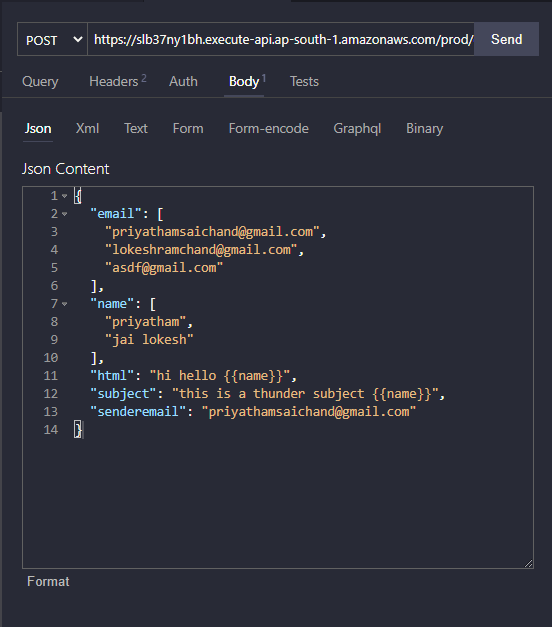
\includegraphics[width=150mm,height=82mm]{figures/api_1.png}
            \caption{Email sending API request}
            \label{fig:email-api}
\end{figure}



In fig \ref{fig:email-api} we show the schema of the request API and all the parameters that needs to be sent. 
\subsection{bounce sending}
We use this API to request the server for the bounce email records that were placed in Dynamo DB.We send a POST request with null parameters and receive the bounce emails. The API end point is given by.

\url{https://slb37ny1bh.execute-api.ap-south-1.amazonaws.com/prod/bounce\_db}

The emails are returned in the form of array of emails and timestamps. Once the bounced emails arrive the delivered emails are computed using the sent emails from the sent email data and the difference of sent and bounced emails gives rise to delivered emails.




\chapter{TESTING AND RESULTS}
\label{ch:testing}

Basic message transfer from Author to Recipients is accomplished by using an asynchronous store-and-forward communication infrastructure in a sequence of independent transmissions through some number of mail transfer agents\cite{rfc5598}. Two of the most common ways to analyze the architecture was to consider the time required to send all the emails and the cost associated with it. Both of the metrics are analysed in the following section.

\section{Performance}
There are two performance monitoring services available to AWS application developers: CloudWatch and X-ray.\cite{lin2018tracking}
 The application is analyzed to see the time required to send the emails and the time taken to run the functions between the request and response to the API endpoint. This can be seen through the cloudwatch\cite{awscloudwatch} logs and X-ray to find out the issues with latency over various regions and finding the best regions and how to optimize the functions.In this case, we used X-Ray as a monitoring and display service that automatically samples the entry and exit of function instances, called segments, using unique trace identifiers \textbf{\texttt{(trace\_id)}}\cite{lin2018tracking}\cite{awsxray}.\par

 Here we take the case of sending multiple emails and the time taken is sampled over 30 data points to represent in Figure 2. The time is calculated by considering the cloudwatch logs that can be used to determine the time taken to execute the last function of lambda as show in Figure 1 to send the email and the time leading to that function from the start of the API gateway request log that is stored in the logs. This experimented several times to cancel out the variations of cold start that is a common phenomenon in serverless functions. All the calculations are done to avoid any overlap between different invocations and only a single request is sent within the same region.\par

\begin{figure}[H]

	\centering
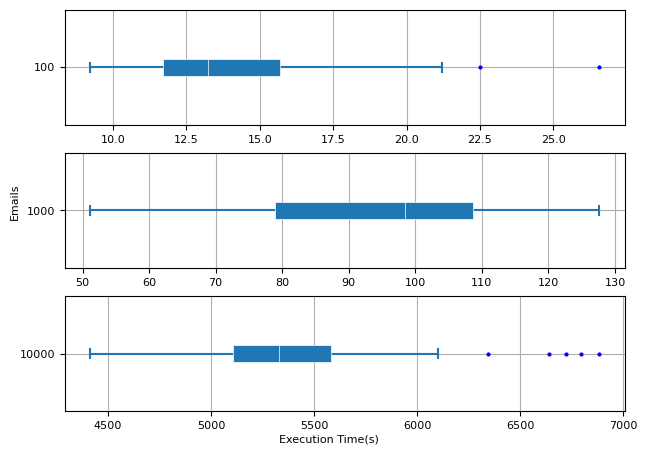
\includegraphics[width=\textwidth]{figures/general_analysis.png}
	\caption{Boxplot depicting the distrubtion of backend runtimes.}
	\label{fig:general}
\end{figure}
In Figure \ref{fig:general} the graph depicts boxplot of runtimes of serverless backend functions after the api is invoked and when email is sent, the number of emails sent is directly proportional to the time taken. The time taken for 10,00 emails averaging at around 30 minutes is sufficient and satisfactory considering that the time taken is to derived from the last email that is sent in the list of emails.  
\section{Error Handling}

Errors in the frontend of the web application is managed by notification pop-up windows that can signify corrections of problems in execution that have occurred.

	

\begin{figure}[H]
\centering
\begin{minipage}[c]{.5\textwidth}
  \centering
  
\includegraphics[width=.9\linewidth]{figures/frontend_error_1.png}
\end{minipage}\hfill
\begin{minipage}[c]{.5\textwidth}
  \centering
  
\includegraphics[width=.9\linewidth]{figures/frontend_errors_2.png}
\end{minipage}\\
\vspace{0.3cm}

\begin{minipage}[c]{.5\textwidth}
  \centering
  
\includegraphics[width=.9\linewidth]{figures/frontend_errors_3.png}
\end{minipage}%
\begin{minipage}[c]{.5\textwidth}
  \centering
  
\includegraphics[width=.9\linewidth]{figures/frontend_errors_4.png}
\end{minipage}\\
\caption{Different Error Messages}
\label{fig:different-errors}
\end{figure}

As shown in Figure \ref{fig:different-errors} If the user leaves out important information that is required by the API. The application halts giving meaningful error messages in a pop-up box at the right corner of screen. 

\section{Cost}
The cost of the services can also be a motivating factor to implement such an architecture. In our use case The following architecture can be tested with the AWS free tier and later expanded to the needs of the users. With \$0.01 dollars per 1,000 emails but one needs to be wary about the associated services like the SES, SNS and the cloudwatch metrics to analyze the emails add up to cost but since they are calculated based on the GB of data it needs to pre-process the rates will not exceed the cost of emails.

Here we take the example, provided by the SES platform to estimate the cost required to implement the architecture.

You use Amazon SES to send about 250,000 emails per month. You receive 1,000 emails per month. You don't use dedicated IP addresses. Every message you send and receive is 32KB in size which results in a total of \$25.98 per month \cite{sespricing} which is significantly less than competitors such as SendGrid or MailChimp who offer their own SMTP server or schedule emails to fit into the constraints of other providers to carry out email campaigns. \par



Amazon provides sample pricing calculations,but as your workload varies, so will the billing. \cite{eivy2017wary} The SQS requests can exceed the free tier if not monitored carefully and add up to additional costs for the next 1000 requests or more based on the usage of the system.\par


\newpage


\section{Results}

The bulk email application has successfully achieved its objective of sending emails in large volumes using the web interface that is provided passing all the test cases and error handling mechanisms. The customization that is proposed is also accomplished by the SES template.

\begin{table}[H]
    \centering
    \begin{tabularx}{.7\textwidth}{| X | X | X | X | X |}
    %\begin{tabularx}{\textwidth}{sssss}
        \hline
        Serial \hspace{0.2cm} Number      & Number of emails     & Mean time taken in (ms) & Median time taken in (ms)\\ \hline
        1         & 100      	  & 14.5        & 13.2     \\ \hline
        2         & 1,000         & 93.4        & 98.4   \\ \hline
        3         & 10,000        & 5511.5       & 5329.9   \\ \hline
    \end{tabularx}
    \caption{Time taken for different volumes of emails}
	    \label{table:time}
\end{table}

In Table \ref{table:time} The time taken by different volumes of email such as 100,1000,1000 taken from the box plot in Figure \ref{fig:general} is used.

\subsection{Dashboard}

The analysis of metrics that are obtained from the sending of emails can be viewed in the form of a high level dashboard and can be shared for real time monitoring of the bounce rate and minimise it and track the success of the email campaign for a specific sending email address.

\begin{figure}[H]
            \centering
            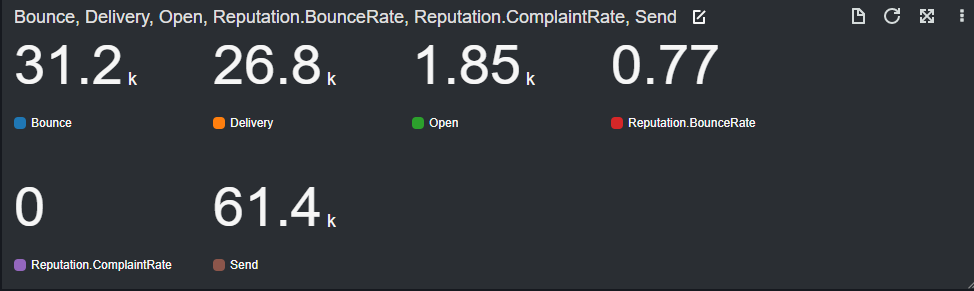
\includegraphics[width=160mm]{figures/dashboard.png}
            \caption{Statistics Dashboard of email services}
	    \label{fig:dashboard}
\end{figure}


As shown the Figure \ref{fig:dashboard}, The various mertrics such as open,sent,delivered,bounced are obtained and are updated in real time with a specific time interval. The duration and time can be changed using filtering options to analyse the campaigns effectively.

\chapter{CONCLUSION AND FUTURE SCOPE}
\label{ch:conclusion}

\section{Conclusion}
To conclude, the architecture has been effective in sending bulk emails of various volumes with runtime that can be considered as sufficient or optimal and cost-effective. The primary goal of the architecture to be able to manage the entire system without a server being provisioned directly i.e. serverless is achieved and is promising to further develop and enhance its capabilities. The statistics displayed can be used for reach through the customers and the key idea of the architecture is to make use of serverless functions and services to manage emails with an optional fronted interface which was the case in this paper. Thus, making it a fast application to deliver emails to the users’ inboxes in a short period of time. Without provisioning any IP addresses and acquiring the compute power needed to send the emails beforehand thereby making it more effective and possesses a higher level of abstraction that the conventional method.

\section{Future Scope}

The following architecture has immense scope to be integrated with various other services such as SMS service or can act as an independent backend logic to implement notficiation service to mobile application for the purposes of marketing or sharing information using other means of communication using the same logic with extensions.


%-----------------------------------------
% References/ Bibliography
%-----------------------------------------

\newpage
\addcontentsline{toc}{chapter}{BIBLIOGRAPHY}
\bibliographystyle{ieeetr}
\bibliography{paper_refs} 


\chapter*{APPENDIX}
\addcontentsline{toc}{chapter}{APPENDIX}

\appendix
\section*{email\_batcher}
\begin{lstlisting}
   var AWS = require('aws-sdk');
AWS.config.update({region: 'ap-south-1'});
var sqs = new AWS.SQS();
var ses = new AWS.SES();
var chunk_size = 50;
exports.handler = async (event,context) => {
// inputs from the request 
    var emails = event['email']
    var names = event['name']
    console.log("received emails: ", emails)
    
    const params1 = {
  Template: {
    TemplateName: "template", 
    HtmlPart: event['html'],
    SubjectPart: event['subject'],
    TextPart: event['html'],
  },
};

try{
var temp =  await ses.createTemplate(params1).promise();
}
catch(error){
console.log("create template ", temp)

    await ses.deleteTemplate({TemplateName: 'template' }).promise();
    await ses.createTemplate(params1).promise();

}

    var emails_count = Object.keys(emails).length;
    var names_count = Object.keys(names).length;
    if(emails_count < names_count)
        return { statusCode: 400, body: 'Error: names are more than emails' }; 
    else{

        var diff = emails_count-names_count;
        for(var i = 0; i < diff; i++){
            names.push('');
        }
    }
// batching the emails
    var final = [];
    var counter = 0;
    var portion = {
        "current_batch": (counter + 1),
        "emails": [],
        "names": [],
        "html": event.html,
        "sender_email": event.senderemail,
        "end_of_batches": false,
    };

     emails.forEach((email,index) => {
         const name = names[index]
         if (counter !== 0 && counter % chunk_size === 0) {
        final.push(portion);
     portion = {
        "current_batch": (counter/2) + 1,
        "emails": [],
        "names": [],
        "html": event.html,
        "sender_email": event.senderemail,
       "end_of_batches": false
    };
      }
      portion['emails'].push(email)
      portion['names'].push(name)
      counter++;
     })
     portion['end_of_batches'] = true
     final.push(portion);

      // sending the batches onto the queue
     var temp = {};
    for (var batch in final){
        var params = {
            MessageGroupId: batch,
      MessageBody: JSON.stringify(final[batch]),
      MessageDeduplicationId: context.getRemainingTimeInMillis().toString(),
      QueueUrl: "https://sqs.ap-south-1.amazonaws.com/285448632456/email_batch.fifo"
    };
       temp = await sqs.sendMessage(params).promise();

    }
    
    return "email sending started";

\end{lstlisting}

\section*{bounce\_emailer}
\begin{lstlisting}
var AWS = require('aws-sdk');
AWS.config.update({region: 'ap-south-1'});
const docClient = new AWS.DynamoDB.DocumentClient();
var sqs = new AWS.SQS();
exports.handler = async (event) => {
   var dest,type; 
    event['Records'].forEach((value,index) =>{
        var message = JSON.parse(value['Sns']['Message'])
        console.log("message: ", message)
        console.log("event type ", message['eventType'])
        dest = message['mail']['destination']
        type = message['bounce']['bounceType']
        console.log("destinations: ", dest)
        
    })
   
   var datetime = new Date();
   const params = {
  TableName : 'emails',
  /* Item properties will depend on your application concerns */
  Item: {
     email: JSON.stringify(dest),
     date: datetime.toISOString(),
     type: type
  }
}
  // run SQL command
   try {
    var temp = await docClient.put(params).promise();
    console.log("success ",temp);
  } catch (err) {
    return err;
  }
    return "function done";
};

\end{lstlisting}

\section*{bounce\_db}
\begin{lstlisting}
var AWS = require('aws-sdk');
AWS.config.update({region: 'ap-south-1'});
const docClient = new AWS.DynamoDB.DocumentClient();

exports.handler = async (event) => {

// retrieve records from db
    const getAllRecords = async (table) => {
  let params = {
    TableName: table,
  };
  let items = [];
  let data = await docClient.scan(params).promise();
  items = [...items, ...data.Items];
  while (typeof data.LastEvaluatedKey != "undefined") {
    params.ExclusiveStartKey = data.LastEvaluatedKey;
    data = await docClient.scan(params).promise();
    items = [...items, ...data.Items];
  }
  return items;
};
const deleteItem = async (table, id) => {
  var params = {
    TableName: table,
    Key: {
      email: id,
    },
  };
  

    let data = await docClient.delete(params).promise();
    return data;
};

var allRecords,allDelete;
// delete records from db
try {
    const tableName = "emails";
    // scan and get all items
     allRecords = await getAllRecords(tableName);
    console.log("records db ", allRecords)
    // delete one by one 
    for (const item of allRecords) {
      allDelete = await deleteItem(tableName, item.email);
    }
  } catch (e) {
      console.log(e)
  }
  
  return allRecords;
};

\end{lstlisting}



\end{document}
